% -*- mode: latex; TeX-master: "Vorbis_I_spec"; -*-
%!TEX root = Vorbis_I_spec.tex
% $Id$
\section{Probability Model and Codebooks} \label{vorbis:spec:codebook}

\subsection{Overview}

Unlike practically every other mainstream audio codec, Vorbis has no
statically configured probability model, instead packing all entropy
decoding configuration, VQ and Huffman, into the bitstream itself in
the third header, the codec setup header.  This packed configuration
consists of multiple 'codebooks', each containing a specific
Huffman-equivalent representation for decoding compressed codewords as
well as an optional lookup table of output vector values to which a
decoded Huffman value is applied as an offset, generating the final
decoded output corresponding to a given compressed codeword.

\subsubsection{Bitwise operation}
The codebook mechanism is built on top of the vorbis bitpacker. Both
the codebooks themselves and the codewords they decode are unrolled
from a packet as a series of arbitrary-width values read from the
stream according to \xref{vorbis:spec:bitpacking}.




\subsection{Packed codebook format}

For purposes of the examples below, we assume that the storage
system's native byte width is eight bits.  This is not universally
true; see \xref{vorbis:spec:bitpacking} for discussion
relating to non-eight-bit bytes.

\subsubsection{codebook decode}

A codebook begins with a 24 bit sync pattern, 0x564342:

\begin{Verbatim}[commandchars=\\\{\}]
byte 0: [ 0 1 0 0 0 0 1 0 ] (0x42)
byte 1: [ 0 1 0 0 0 0 1 1 ] (0x43)
byte 2: [ 0 1 0 1 0 1 1 0 ] (0x56)
\end{Verbatim}

16 bit \varname{[codebook\_dimensions]} and 24 bit \varname{[codebook\_entries]} fields:

\begin{Verbatim}[commandchars=\\\{\}]

byte 3: [ X X X X X X X X ]
byte 4: [ X X X X X X X X ] [codebook\_dimensions] (16 bit unsigned)

byte 5: [ X X X X X X X X ]
byte 6: [ X X X X X X X X ]
byte 7: [ X X X X X X X X ] [codebook\_entries] (24 bit unsigned)

\end{Verbatim}

Next is the \varname{[ordered]} bit flag:

\begin{Verbatim}[commandchars=\\\{\}]

byte 8: [               X ] [ordered] (1 bit)

\end{Verbatim}

Each entry, numbering a
total of \varname{[codebook\_entries]}, is assigned a codeword length.
We now read the list of codeword lengths and store these lengths in
the array \varname{[codebook\_codeword\_lengths]}. Decode of lengths is
according to whether the \varname{[ordered]} flag is set or unset.

\begin{itemize}
\item
  If the \varname{[ordered]} flag is unset, the codeword list is not
  length ordered and the decoder needs to read each codeword length
  one-by-one.

  The decoder first reads one additional bit flag, the
  \varname{[sparse]} flag.  This flag determines whether or not the
  codebook contains unused entries that are not to be included in the
  codeword decode tree:

\begin{Verbatim}[commandchars=\\\{\}]
byte 8: [             X 1 ] [sparse] flag (1 bit)
\end{Verbatim}

  The decoder now performs for each of the \varname{[codebook\_entries]}
  codebook entries:

\begin{Verbatim}[commandchars=\\\{\}]

  1) if([sparse] is set) \{

         2) [flag] = read one bit;
         3) if([flag] is set) \{

              4) [length] = read a five bit unsigned integer;
              5) codeword length for this entry is [length]+1;

            \} else \{

              6) this entry is unused.  mark it as such.

            \}

     \} else the sparse flag is not set \{

        7) [length] = read a five bit unsigned integer;
        8) the codeword length for this entry is [length]+1;

     \}

\end{Verbatim}

\item
  If the \varname{[ordered]} flag is set, the codeword list for this
  codebook is encoded in ascending length order.  Rather than reading
  a length for every codeword, the encoder reads the number of
  codewords per length.  That is, beginning at entry zero:

\begin{Verbatim}[commandchars=\\\{\}]
  1) [current\_entry] = 0;
  2) [current\_length] = read a five bit unsigned integer and add 1;
  3) [number] = read \link{vorbis:spec:ilog}{ilog}([codebook\_entries] - [current\_entry]) bits as an unsigned integer
  4) set the entries [current\_entry] through [current\_entry]+[number]-1, inclusive,
    of the [codebook\_codeword\_lengths] array to [current\_length]
  5) set [current\_entry] to [number] + [current\_entry]
  6) increment [current\_length] by 1
  7) if [current\_entry] is greater than [codebook\_entries] ERROR CONDITION;
    the decoder will not be able to read this stream.
  8) if [current\_entry] is less than [codebook\_entries], repeat process starting at 3)
  9) done.
\end{Verbatim}

\end{itemize}

After all codeword lengths have been decoded, the decoder reads the
vector lookup table.  Vorbis I supports three lookup types:
\begin{enumerate}
\item
No lookup
\item
Implicitly populated value mapping (lattice VQ)
\item
Explicitly populated value mapping (tessellated or 'foam'
VQ)
\end{enumerate}


The lookup table type is read as a four bit unsigned integer:
\begin{Verbatim}[commandchars=\\\{\}]
  1) [codebook\_lookup\_type] = read four bits as an unsigned integer
\end{Verbatim}

Codebook decode precedes according to \varname{[codebook\_lookup\_type]}:
\begin{itemize}
\item
Lookup type zero indicates no lookup to be read.  Proceed past
lookup decode.
\item
Lookup types one and two are similar, differing only in the
number of lookup values to be read.  Lookup type one reads a list of
values that are permuted in a set pattern to build a list of vectors,
each vector of order \varname{[codebook\_dimensions]} scalars.  Lookup
type two builds the same vector list, but reads each scalar for each
vector explicitly, rather than building vectors from a smaller list of
possible scalar values.  Lookup decode proceeds as follows:

\begin{Verbatim}[commandchars=\\\{\}]
  1) [codebook\_minimum\_value] = \link{vorbis:spec:float32:unpack}{float32\_unpack}( read 32 bits as an unsigned integer)
  2) [codebook\_delta\_value] = \link{vorbis:spec:float32:unpack}{float32\_unpack}( read 32 bits as an unsigned integer)
  3) [codebook\_value\_bits] = read 4 bits as an unsigned integer and add 1
  4) [codebook\_sequence\_p] = read 1 bit as a boolean flag

  if ( [codebook\_lookup\_type] is 1 ) \{

     5) [codebook\_lookup\_values] = \link{vorbis:spec:lookup1:values}{lookup1\_values}(\varname{[codebook\_entries]}, \varname{[codebook\_dimensions]} )

  \} else \{

     6) [codebook\_lookup\_values] = \varname{[codebook\_entries]} * \varname{[codebook\_dimensions]}

  \}

  7) read a total of [codebook\_lookup\_values] unsigned integers of [codebook\_value\_bits] each;
     store these in order in the array [codebook\_multiplicands]
\end{Verbatim}
\item
A \varname{[codebook\_lookup\_type]} of greater than two is reserved
and indicates a stream that is not decodable by the specification in this
document.

\end{itemize}


An 'end of packet' during any read operation in the above steps is
considered an error condition rendering the stream undecodable.

\paragraph{Huffman decision tree representation}

The \varname{[codebook\_codeword\_lengths]} array and
\varname{[codebook\_entries]} value uniquely define the Huffman decision
tree used for entropy decoding.

Briefly, each used codebook entry (recall that length-unordered
codebooks support unused codeword entries) is assigned, in order, the
lowest valued unused binary Huffman codeword possible.  Assume the
following codeword length list:

\begin{Verbatim}[commandchars=\\\{\}]
entry 0: length 2
entry 1: length 4
entry 2: length 4
entry 3: length 4
entry 4: length 4
entry 5: length 2
entry 6: length 3
entry 7: length 3
\end{Verbatim}

Assigning codewords in order (lowest possible value of the appropriate
length to highest) results in the following codeword list:

\begin{Verbatim}[commandchars=\\\{\}]
entry 0: length 2 codeword 00
entry 1: length 4 codeword 0100
entry 2: length 4 codeword 0101
entry 3: length 4 codeword 0110
entry 4: length 4 codeword 0111
entry 5: length 2 codeword 10
entry 6: length 3 codeword 110
entry 7: length 3 codeword 111
\end{Verbatim}


\begin{note}
Unlike most binary numerical values in this document, we
intend the above codewords to be read and used bit by bit from left to
right, thus the codeword '001' is the bit string 'zero, zero, one'.
When determining 'lowest possible value' in the assignment definition
above, the leftmost bit is the MSb.
\end{note}

It is clear that the codeword length list represents a Huffman
decision tree with the entry numbers equivalent to the leaves numbered
left-to-right:

\begin{center}
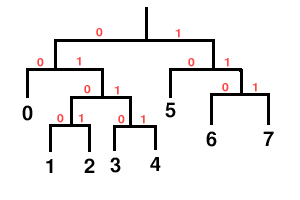
\includegraphics[width=10cm]{hufftree}
\captionof{figure}{huffman tree illustration}
\end{center}


As we assign codewords in order, we see that each choice constructs a
new leaf in the leftmost possible position.

Note that it's possible to underspecify or overspecify a Huffman tree
via the length list.  In the above example, if codeword seven were
eliminated, it's clear that the tree is unfinished:

\begin{center}
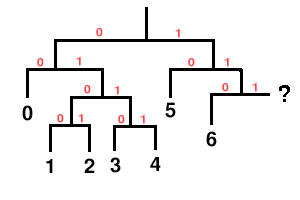
\includegraphics[width=10cm]{hufftree-under}
\captionof{figure}{underspecified huffman tree illustration}
\end{center}


Similarly, in the original codebook, it's clear that the tree is fully
populated and a ninth codeword is impossible.  Both underspecified and
overspecified trees are an error condition rendering the stream
undecodable. Take special care that a codebook with a single used
entry is handled properly; it consists of a single codework of zero
bits and 'reading' a value out of such a codebook always returns the
single used value and sinks zero bits.  

Codebook entries marked 'unused' are simply skipped in the assigning
process.  They have no codeword and do not appear in the decision
tree, thus it's impossible for any bit pattern read from the stream to
decode to that entry number.



\paragraph{VQ lookup table vector representation}

Unpacking the VQ lookup table vectors relies on the following values:
\begin{programlisting}
the [codebook\_multiplicands] array
[codebook\_minimum\_value]
[codebook\_delta\_value]
[codebook\_sequence\_p]
[codebook\_lookup\_type]
[codebook\_entries]
[codebook\_dimensions]
[codebook\_lookup\_values]
\end{programlisting}

\bigskip

Decoding (unpacking) a specific vector in the vector lookup table
proceeds according to \varname{[codebook\_lookup\_type]}.  The unpacked
vector values are what a codebook would return during audio packet
decode in a VQ context.

\paragraph{Vector value decode: Lookup type 1}

Lookup type one specifies a lattice VQ lookup table built
algorithmically from a list of scalar values.  Calculate (unpack) the
final values of a codebook entry vector from the entries in
\varname{[codebook\_multiplicands]} as follows (\varname{[value\_vector]}
is the output vector representing the vector of values for entry number
\varname{[lookup\_offset]} in this codebook):

\begin{Verbatim}[commandchars=\\\{\}]
  1) [last] = 0;
  2) [index\_divisor] = 1;
  3) iterate [i] over the range 0 ... [codebook\_dimensions]-1 (once for each scalar value in the value vector) \{

       4) [multiplicand\_offset] = ( [lookup\_offset] divided by [index\_divisor] using integer
          division ) integer modulo [codebook\_lookup\_values]

       5) vector [value\_vector] element [i] =
            ( [codebook\_multiplicands] array element number [multiplicand\_offset] ) *
            [codebook\_delta\_value] + [codebook\_minimum\_value] + [last];

       6) if ( [codebook\_sequence\_p] is set ) then set [last] = vector [value\_vector] element [i]

       7) [index\_divisor] = [index\_divisor] * [codebook\_lookup\_values]

     \}

  8) vector calculation completed.
\end{Verbatim}



\paragraph{Vector value decode: Lookup type 2}

Lookup type two specifies a VQ lookup table in which each scalar in
each vector is explicitly set by the \varname{[codebook\_multiplicands]}
array in a one-to-one mapping.  Calculate [unpack] the
final values of a codebook entry vector from the entries in
\varname{[codebook\_multiplicands]} as follows (\varname{[value\_vector]}
is the output vector representing the vector of values for entry number
\varname{[lookup\_offset]} in this codebook):

\begin{Verbatim}[commandchars=\\\{\}]
  1) [last] = 0;
  2) [multiplicand\_offset] = [lookup\_offset] * [codebook\_dimensions]
  3) iterate [i] over the range 0 ... [codebook\_dimensions]-1 (once for each scalar value in the value vector) \{

       4) vector [value\_vector] element [i] =
            ( [codebook\_multiplicands] array element number [multiplicand\_offset] ) *
            [codebook\_delta\_value] + [codebook\_minimum\_value] + [last];

       5) if ( [codebook\_sequence\_p] is set ) then set [last] = vector [value\_vector] element [i]

       6) increment [multiplicand\_offset]

     \}

  7) vector calculation completed.
\end{Verbatim}









\subsection{Use of the codebook abstraction}

The decoder uses the codebook abstraction much as it does the
bit-unpacking convention; a specific codebook reads a
codeword from the bitstream, decoding it into an entry number, and then
returns that entry number to the decoder (when used in a scalar
entropy coding context), or uses that entry number as an offset into
the VQ lookup table, returning a vector of values (when used in a context
desiring a VQ value). Scalar or VQ context is always explicit; any call
to the codebook mechanism requests either a scalar entry number or a
lookup vector.

Note that VQ lookup type zero indicates that there is no lookup table;
requesting decode using a codebook of lookup type 0 in any context
expecting a vector return value (even in a case where a vector of
dimension one) is forbidden.  If decoder setup or decode requests such
an action, that is an error condition rendering the packet
undecodable.

Using a codebook to read from the packet bitstream consists first of
reading and decoding the next codeword in the bitstream. The decoder
reads bits until the accumulated bits match a codeword in the
codebook.  This process can be though of as logically walking the
Huffman decode tree by reading one bit at a time from the bitstream,
and using the bit as a decision boolean to take the 0 branch (left in
the above examples) or the 1 branch (right in the above examples).
Walking the tree finishes when the decode process hits a leaf in the
decision tree; the result is the entry number corresponding to that
leaf.  Reading past the end of a packet propagates the 'end-of-stream'
condition to the decoder.

When used in a scalar context, the resulting codeword entry is the
desired return value.

When used in a VQ context, the codeword entry number is used as an
offset into the VQ lookup table.  The value returned to the decoder is
the vector of scalars corresponding to this offset.
